\chapter{Revisão de mecânica}\label{capitulo:revisao_mecanica}

Este capítulo tem como objetivo apresentar brevemente conceitos importantes da mecânica analítica, com foco na formulação hamiltoniana. Apesar do foco central deste trabalho ser a simulação do Problema de N-Corpos Gravitacional (PNCG), a maior parte do conteúdo aqui apresentado se aplica a outros problemas físicos graças à solidez teórica da mecânica analítica.

Partiremos da Mecânica Newtoniana e de seus conceitos fundamentais, atravessaremos rapidamente a Mecânica Lagrangiana e através da transformação de Legendre seremos levados às equações de Hamilton, as quais abrem as portas para a Mecânica Hamiltoniana.

O PNCG é um problema mecânico conservativo, então nas simulações utilizamos muito frequentemente os métodos chamados \textit{simpléticos}, apresentados no capítulo \ref{capitulo:metodos_numericos}. Por isso, uma parte considerável deste capítulo de mecânica é destinado à apresentação da teoria de formas diferenciais, o básico da geometria simplética e a teoria de transformações canônicas.

\section{De Newton a Lagrange}

Nesta seção, são revisados brevemente conceitos de Mecânica Newtoniana e de Mecânica Lagrangiana, partindo da 2ª Lei de Newton, passando por integrais primeiras, o funcional de ação, funções lagrangianas e encerrando com a Transformação de Legendre e as Equações de Hamilton. O intuito é dar base para a seção seguinte, relativa a Mecânica Hamiltoniana.

\subsection{Equações de movimento na mecânica newtoniana}
Na mecânica newtoniana, os objetos são descritos matematicamente a partir de dois referenciais absolutos: o espaço e o tempo. As equações de movimento que parametrizam tais objetos são dadas pela 2ª Lei de Newton.

\begin{definition}[2ª Lei de Newton]
    Um objeto de massa $m > 0$, posição inicial $\vet q_0 \in M \subseteq \R^n$ e sujeito a um campo de forças $\vet F: I \times M \to M$, $I \subseteq \R$, tem sua trajetória $\vet q: I \subseteq \R \to M$ descrita pelo seguinte Problema de Cauchy:
    \begin{equation}\label{eq:segunda_lei_de_newton}
        \begin{cases}
            m \ddvet q (t) = \vet F(t, \vet q(t)), \forall t \in I, \\
            \vet q(t_0) = \vet q_0, \dvet q(t_0) = \dvet q_0, \ t_0 \in I.
        \end{cases}
    \end{equation}
\end{definition}

No caso do PNCG, tratado com detalhes no capítulo \ref{capitulo:pncg}, o campo de forças depende somente da posição, e como as equações são autônomas (isto é, não dependem explicitamente do tempo), escrevemos na forma de notação reduzida:
\begin{equation}
    m \ddvet q = F(\vet q),
\end{equation}
ou, ainda, tomando $\vet v(t) \in T_{\vet q(t)} M$, onde $T_{\vet q(t)} M$ é o espaço tangente a $M$ em $\vet q(t)$\footnote{Os conceitos de espaços e fibrados tangente e cotangente são melhor explorados na seção \ref{subsecao:k-formas}. No momento, para visualizar $TM$ qualquer basta pensar em uma derivada temporal.}, e definindo $\vet v_0 = \vet v(t_0)$, podemos escrever na seguinte forma:
\begin{equation}
    \begin{cases}
        \dvet q = \vet v, \\
        \dvet v = \frac{1}{m} \vet F(\vet q), \\
        \vet q(t_0) = \vet q_0, \vet v(t_0) = \vet v_0.
    \end{cases}
\end{equation}

Nos sistemas newtonianos, um conceito que aparece naturalmente é a energia total.

\begin{definition}[Função potencial]
    Quando $\vet F$ é um campo gradiente, isto é, existe uma função suave $V:M \to \R$ tal que $\vet F = - \nabla V$, dizemos que $V$ é uma \textbf{função potencial} do sistema.
\end{definition}

\begin{definition}[Energia total]
    A energia total $E$ de um sistema newtoniano com função potencial $V$ é dada por
    \begin{equation}\label{eq:energia_total}
        E(t, \vet q, \vet v) = \dfrac{1}{2} m \norma{\vet v}^2 + V(\vet q),
    \end{equation}
    onde $\frac{1}{2} m \norma{\vet v}^2$ é chamada de \textbf{energia cinética} e a função potencial é chamada de \textbf{energia potencial}.
\end{definition}

A energia total, quando não depende explicitamente do tempo e o campo é fechado (ou seja, não há forçantes), possui a propriedade de ser uma \textit{integral primeira} do sistema, isto é, é constante em relação ao tempo.

\begin{definition}[Integral primeira]\label{def:integral_primeira}
    Um observável $f$ (uma função que depende de $t$, $\vet q$ e $\vet v$) é dito uma \textbf{integral primeira} se for pelo menos $\continuo^1$ e
    \begin{equation}
        \der{}{t} f (t, \vet q(t), \vet v(t)) = 0, \forall t \in I.
    \end{equation}
\end{definition}

\begin{theorem}\label{teorema:energia_total}
    A energia total $E(t, \vet q(t), \vet v(t))$ de um sistema newtoniano é uma integral primeira.
\end{theorem}
\begin{Proof}
    Basta derivar:
    \begin{align*}
        \der{}{t} E(t, \vet q(t), \vet v(t))
        &= \dfrac{1}{2} m \der{}{t}(\norma{\vet v}^2) + \der{}{t} V(\vet q(t))  \\
        &= \dfrac{1}{2} m 2 \prodint{\vet v}{\dvet v} + \prodint{\nabla V}{\vet v} \\
        &= \prodint{\vet v}{\vet F} - \prodint{\vet F}{\vet v} = 0.
    \end{align*}
\end{Proof}

Isso significa que a partir de um par de valores iniciais $(\vet q_0, \vet v_0)$, obtém-se a energia total de toda a trajetória. Analiticamente, quando um sistema em $\R^n$ possui $k$-integrais primeiras não-triviais, é possível remodelar o sistema para trabalhar em um espaço reduzido $\R^{n-k}$ \citep[93-94]{de_queiroz_barros_mecanica_1995}. Já numericamente, isso é interessante do ponto de vista da precisão numérica, pois, uma vez que a energia deve se manter constante durante a trajetória, sua variação numérica é uma forma de mensurar os erros nas aproximações.

\subsection{Ação e Lagrangianos}
Na modelagem obtida, as trajetórias dos objetos são descritas localmente, pois as equações de movimento muitas vezes não possuem soluções para todo $t \in \R$, estando no geral definidas apenas na vizinhança do instante inicial.

Para movimentos em circuitos definidos em espaços conexos, existe ao menos uma curva ligando os pontos inicial e final. O critério para determinar qual curva corresponde a um dado conjunto de valores iniciais é dado a partir de uma métrica e, com ela, a atribuição de um valor real a cada curva $\gamma(t) = (\vet q(t), \vet v(t))$ em $[t_0,t_f]$, o que pode ser feito da seguinte maneira:
\begin{equation}
    S(\gamma) = \int_{t_0}^{t_f} L(\gamma(t)) dt = \int_{t_0}^{t_f} L(\vet q(t), \vet v(t)) dt.
\end{equation}

Aqui $S$ é um funcional chamado \textit{ação} e $L$ é uma função que a princípio pode ser qualquer. Tomando $L(\vet q(t), \vet v(t)) = \sqrt{1 + \vet v(t)}$, por exemplo, $S$ mede o comprimento de $\gamma$.

Podemos definir uma \textit{aproximação} ou \textit{deformação} $\tilde \gamma$ de $\gamma$ como $\tilde \gamma (t) = \gamma(t) + h(t)$, para alguma curva $h$ definida no mesmo espaço de $\gamma$.

\begin{definition}
    Um funcional $\Phi$ é dito \textit{diferenciável} se $\Phi(\gamma + h) - \Phi(\gamma) = F + R$, onde $F$ depende linearmente de $h$ e $R(h, \gamma) = O(h^2)$, no sentido de que, para $|h| < \epsilon$ e $|dh/dt| < \epsilon$, temos $|R| < C \epsilon^2$. A parte linear $F(h)$ é chamada de \textit{diferencial}.
\end{definition}

\begin{theorem}\label{teorema:derivada_acao}
    O funcional de ação é diferenciável, e seu diferencial é dado por
    \begin{equation}
        F(h) = \int_{t_0}^{t_f} \left[ \derpar{L}{\vet q} - \der{}{t} \derpar{L}{\vet v} \right] h dt
    \end{equation}
\end{theorem}
\begin{Proof}
    Temos que:
    \begin{align*}
        S(\gamma + h) - S(\gamma) 
        &= \int_{t_0}^{t_f} [L(\vet q + h, \vet v + \dot h) - L(\vet q, \vet v)] dt \\
        &= \int_{t_-0}^{t_f} \left[\derpar{L}{\vet q} h + \derpar{L}{\vet v} \dot h\right] dt + O(h^2) = F(h) + R,
    \end{align*}
    pois
    \begin{equation*}
        L(\vet q + h, \vet v + \dot h) = L(\vet q, \vet v) + \prodint{(h, \dot h)}{\nabla L(\vet q, \vet v)} + O(h^2).
    \end{equation*}
    Integrando por partes, obtemos:
    \begin{equation*}
        \int_{t_0}^{t_f} \derpar{L}{\vet v} \dot h dt =
        - \int_{t_0}^{t_f} h \der{}{t} \left(\derpar{L}{\vet v}\right) dt + \left(h \derpar{L}{\vet v} \right)\bigg\rvert_{t_0}^{t_f}.
    \end{equation*}
    Uma vez que $h(t_0) = h(t_f) = 0$ (pela definição de deformação), então obtemos o esperado.
\end{Proof}

A partir do conceito de diferencial, é intuitiva a definição de \textit{extremos} ou \textit{curvas críticas}, análoga ao conceito de \textit{pontos críticos} de funções, sendo ``pontos'' (em um espaço de funções) que maximizam ou minimizam o funcional.

\begin{definition}
    Um \textit{extremo} de um funcional diferenciável $\Phi(\gamma)$ é uma curva $\gamma$ tal que $F(h, \gamma) = 0$, para todo $h$.
\end{definition}

\begin{theorem}
    A curva $\gamma$ é um extremo de $S$ se, e somente se,
    \begin{equation}\label{eq:euler_lagrange}
        \derpar{L}{\vet q} - \der{}{t}\left(\derpar{L}{\vet v}\right) = 0, \quad \forall t \in [t_0, t_f].
    \end{equation}
\end{theorem}
\begin{Proof}
    Pelo teorema \ref{teorema:derivada_acao}, $F(h) = 0$ se e somente se $h = 0$ ou
    \begin{equation*}
        \derpar{L}{\vet q} - \der{}{t}\left(\derpar{L}{\vet v}\right) = 0.
    \end{equation*}
    Uma vez que $h \neq 0$ (pois é uma deformação), temos o esperado.
\end{Proof}

A equação (\ref{eq:euler_lagrange}) é chamada de \textit{Equação de Euler-Lagrange}. Essa equação, munida do \textit{Princípio de Hamilton}, caracteriza o movimento na mecânica lagrangiana.

\begin{theorem}[Princípio de Hamilton]
    A 2ª Lei de Newton em (\ref{eq:segunda_lei_de_newton}) coincide com extremos do funcional de ação
    \begin{equation*}
        S(\gamma) = \int_{t_0}^{t_f} L \ dt,
    \end{equation*}
    onde $L = T - V$ é a diferença entre as energias cinética e potencial.
\end{theorem}
\begin{Proof}
    Basta derivar:
    \begin{equation*}
        \derpar{L}{\vet q} = - \derpar{V}{\vet q},
        \quad
        \derpar{L}{\vet v} = \derpar{}{\vet v}\left(\dfrac{1}{2} m \vet v^2 \right) = m \vet v
        \Rightarrow
        \der{}{t}(m \vet v) = -\derpar{V}{\vet q} = F(\vet q).
    \end{equation*}
\end{Proof}

\begin{definition}\label{def:generalizados}
    A função $L(\vet q, \vet v) = \frac{1}{2} m \vet v^2 - V$ é a \textbf{função lagrangiana} ou \textbf{lagrangiano} do sistema, $\vet q$ são as \textbf{coordenadas generalizadas}, $\vet v$ são as \textbf{velocidades generalizadas}, $\partial L / \partial \vet v = \vet p$ são os \textbf{momentos generalizados} e $\partial L / \partial \vet q$ são as \textbf{forças generalizadas}.
\end{definition}

A mecânica lagrangiana é amplamente utilizada para modelar diversos problemas, desde sistemas mecânicos simples com vínculos até o próprio Modelo Padrão de partículas. No entanto, para o PNCG há uma formulação mais interessante que é a \textit{mecânica hamiltoniana}. Ainda assim, o conceito de ação é relevante, como por exemplo na formulação da \textit{Dinâmica de Formas}, apresentada brevemente na seção \ref{secao:dinamica_de_formas}.

\subsection{Transformação de Legendre e Equações de Hamilton}

Observe que até então o par considerado era $(\vet q, \vet v)$, ou seja, pontos no fibrado tangente de $M$. Na definição \ref{def:generalizados} foi apresentado o conceito de momento generalizado, e o par $(\vet q, \vet p)$ se encontra no fibrado cotangente de $M$. Tal construção de coordenadas é explorada com um pouco mais de detalhes na seção \ref{secao:mecanica_hamiltoniana}. Para o que interessa agora, a transformação de Legendre é uma aplicação entre os dois espaços.

\begin{definition}
    Sejam $U \subseteq \R^n \times \R^m$ aberto e $X:U \to \R$ de classe $\continuo^{k+2}$. Dizemos que $X$ é \textbf{Legendre transformável} em $x$ se a aplicação
    \begin{equation*}
        F:(\alpha, x) \in U \quad \mapsto \quad (\alpha, y) \in \R^n \times \R^m
    \end{equation*}
    definida por
    \begin{equation*}
        y = \derpar{X}{x}(x, \alpha), \quad \alpha = \alpha
    \end{equation*}
    é um difeomorfismo $\continuo^{k+1}$ sobre a imagem $F(U)$.
\end{definition}

\begin{definition}
    Considere $X$ Legendre transformável, nos mesmos espaços. A aplicação $Y:V \to \R$ definida por
    \begin{equation*}
        (\alpha, y) = F(\alpha, x) \quad \Rightarrow \quad X(\alpha, x) + Y(\alpha, y) = \prodint{x}{y}
    \end{equation*}
    é chamada \textit{transformada de Legendre de $X$}.
    De maneira explícita:
    \begin{equation*}
        Y(y, \alpha) = (F^{-1})(y, \alpha) y - X(F^{-1}(y, \alpha)),
    \end{equation*}
    e a transformação $y = \partial X/\partial x$ é chamada \textbf{transformação de Legendre}.
\end{definition}

É mister observar que a transformada de Legendre é involutiva, ou seja, se $X$ é Legendre transformável com transformada $Y$, então $Y$ é Legendre transformável com transformada $X$ \citep[79]{de_queiroz_barros_mecanica_1995}. Além disso, trata-se de uma aplicação que leva uma função a um funcional linear definido no dual do espaço original.

Partindo de Lagrange, a função lagrangiana $L = \frac{1}{2} m \vet v^2 - V$ é uma função suave, uma vez que $V$ é suave, e o momento generalizado também o é, então a aplicação que leva $(\vet q, \vet v)$ em $(\vet q, \vet p)$ é um difeomorfismo suave. Assim, $L$ é uma função Legendre transformável em relação a $\vet v$.

\begin{definition}[Função hamiltoniana]
    A transformada de Legendre $H$ de $L$ é chamada de \textit{função hamiltoniana} e é dada por
    \begin{equation}\label{eq:legendre_hamilton}
        H(\vet q, \vet p) = \prodint{\vet v}{\vet p} - L(\vet q, \vet v)
    \end{equation}
\end{definition}

\begin{observation}
    Quando $L = \frac{1}{2} m \vet v^2 - V$, a função hamiltoniana corresponde à energia total como definida em (\ref{eq:energia_total}), pois
    \begin{equation*}
        H = \prodint{\vet v}{\vet p} - L 
        = \prodint{\vet v}{\derpar{L}{\vet v}} - \frac{1}{2} m \vet v^2 + V
        = m \norma{\vet v}^2 - \frac{1}{2} m \vet v^2 + V
        = \frac{1}{2 m} \vet p^2 + V.
    \end{equation*}
    Aqui, a energia cinética pode ser escrita em função do momento generalizado:
    \begin{equation}
        T(\vet p) = \dfrac{\vet p^2}{2m}.
    \end{equation}
\end{observation}

Enquanto $L$ está definida sobre o fibrado tangente $TM$, $H$ estará definida sobre o fibrado cotangente $T^*M$, que é o fibrado dual de $TM$ \citep[192]{Tu2010-sb}. A função hamiltoniana também fornece um novo conjunto de equações de movimento, chamadas \textit{equações de Hamilton}.

\begin{theorem}[Equações de Hamilton]\label{teorema:equacoes_hamilton}
    A função hamiltoniana gera as seguintes equações de movimento:
    \begin{equation*}
        \der{\vet q}{t} = \derpar{H}{\vet p},
        \quad
        \der{\vet p}{t} = - \derpar{H}{\vet q}.
    \end{equation*}
\end{theorem}
\begin{Proof}
    Basta derivar (\ref{eq:legendre_hamilton}):
    \begin{align*}
        \derpar{H}{\vet q} = -\derpar{L}{\vet q} = \derpar{V}{\vet q} = - \dvet p, \quad
        \derpar{H}{\vet p} = \vet v - \left(\vet p - \derpar{L}{\vet v}\right) \derpar{\vet v}{\vet p} = \vet v = \dvet q.
    \end{align*}
\end{Proof}

Definindo $\vet z = (\vet q, \vet p)$, há uma forma reduzida para as equações de Hamilton:
\begin{equation*}
    \dvet z(t) = \begin{bmatrix}
        \vet 0 & \vet I \\ - \vet I & \vet 0
    \end{bmatrix}
    \nabla_{\vet z} H(\vet z(t))
    = \bm \Omega \nabla_{\vet z} H(\vet z(t)),
\end{equation*}
onde $\bm \Omega$ é chamada \textbf{matriz simplética}. Este nome será justificado na próxima seção.

A importância da formulação hamiltoniana começa a aparecer a partir do seguinte teorema.

\begin{theorem}\label{teorema:hamiltoniano_volume}
    O fluxo hamiltoniano $\varphi = (\vet q, \vet p)$ dado por $\der{}{t} \varphi = V$, onde $V = (\dvet q, \dvet p) = (\nabla_{\vet p} H, - \nabla_{\vet q} H)$, conserva volume.
\end{theorem}

Antes de prová-lo, é necessário um lema.

\begin{lemma}\label{lema:divergente_volume}
    Sejam $\varphi: I \subseteq \R \to \R^n$ e $F: \R^n \to \R^n$ tais que
    \begin{equation*}
        \der{\varphi}{t} = F(\varphi(t)),
    \end{equation*}
    e suponha que $\nabla \cdot F = 0$. Então sendo $R_0 \subseteq \R^n$ uma região compacta cuja evolução é dada por $R(t) = \{\varphi(t) | \varphi(0) \in R_0\}$, o volume de $R(t)$ é constante no tempo. 
\end{lemma}
\begin{Proof}
    O volume $V(t)$ de $R(t)$ é dado por
    \begin{equation*}
        V(t) = \int_{R(t)} d\vet x.
    \end{equation*}
    Assim, para um pequeno $dt > 0$, tem-se que
    \begin{equation*}
        V(t+dt) = \int_{R(t)} \det{\derpar{\varphi_i(t+dt)}{\varphi_j(t)}} d\vet x,
    \end{equation*}
    onde o último termo é o determinante da matriz jacobiana da aplicação que leva $\varphi(t)$ a $\varphi(t+dt)$, dada a mudança de coordenadas imposta. Pela definição de derivada,
    \begin{equation*}
        \varphi_i(t+dt) = \varphi_i(t) + V_i(\varphi(t)) dt + O(dt^2),
    \end{equation*}
    logo
    \begin{equation*}
        \derpar{\varphi_i(t+dt)}{\varphi_j(t)} = \delta_{ij} + \derpar{V_i}{x_j} dt + O(dt^2).
    \end{equation*}

    Considere agora uma matriz $A$ qualquer, com autovalores $\lambda_i$. A matriz $I + \epsilon A$, para $\epsilon$ suficientemente pequeno, terá autovalores $1 + \epsilon \lambda_i$. Dessa forma, tem-se que:
    \begin{equation*}
        \det{\left(I + \epsilon A \right)} = \prod (1 + \epsilon \lambda_i) = 1 + \epsilon \sum_i \lambda_i + O(\epsilon^2) = 1 + \epsilon \Tr A + O(\epsilon^2).
    \end{equation*}

    Dessa forma, o volume $V(t+dt)$ pode ser escrito como
    \begin{align*}
        V(t+dt) &= \int_{R(t)} \left\lvert \delta_i^j + \derpar{V_i}{x_j}dt + O(dt^2) \right\rvert d\vet x\\
        &= \int_{R(t)} \left(1 + \nabla \cdot V dt + O(dt^2) \right) d\vet x \\
        &= V(t) + \int_{R(t)} (\nabla \cdot V dt) d\vet x + O(dt^2) \\
        \therefore \der{V}{t} &= \int_{R(t)} \nabla \cdot V d\vet x.
    \end{align*}

    Assim, se $\nabla \cdot V = 0$, volume do fluxo não varia com o tempo.    
\end{Proof}

\begin{Proof} (Do teorema)
    Conforme o lema \ref{lema:divergente_volume}, basta verificar que o divergente do campo hamiltoniano é nulo.
    \begin{equation*}
        \nabla \cdot V 
        = \derpar{\dvet q}{\vet q} + \derpar{\dvet p}{\vet p}
        = \dfrac{\partial^2 H}{\partial \vet q \partial \vet p} - \dfrac{\partial^2 H}{\partial \vet p \partial \vet q} = 0,
    \end{equation*}
    pois $H$ é suave.
\end{Proof}

Isso significa que no espaço das coordenadas $(\vet q, \vet p)$, também chamado de \textit{espaço de fases}, o fluxo tem seu volume conservado na órbita das soluções.

% \subsection{Equações de movimento na mecânica newtoniana}
Na mecânica newtoniana, os objetos são descritos matematicamente a partir de dois referenciais absolutos: o espaço e o tempo. As equações de movimento que parametrizam tais objetos são dadas pela 2ª Lei de Newton.

\begin{definition}[2ª Lei de Newton]
    Um objeto de massa $m > 0$, posição inicial $\vet q_0 \in M \subseteq \R^n$ e sujeito a um campo de forças $\vet F: I \times M \to M$, $I \subseteq \R$, tem sua trajetória $\vet q: I \subseteq \R \to M$ descrita pelo seguinte Problema de Cauchy:
    \begin{equation}\label{eq:segunda_lei_de_newton}
        \begin{cases}
            m \ddvet q (t) = \vet F(t, \vet q(t)), \forall t \in I, \\
            \vet q(t_0) = \vet q_0, \dvet q(t_0) = \dvet q_0, \ t_0 \in I.
        \end{cases}
    \end{equation}
\end{definition}

No caso do PNCG, tratado com detalhes no capítulo \ref{capitulo:pncg}, o campo de forças depende somente da posição, e como as equações são autônomas (isto é, não dependem explicitamente do tempo), escrevemos na forma de notação reduzida:
\begin{equation}
    m \ddvet q = F(\vet q),
\end{equation}
ou, ainda, tomando $\vet v(t) \in T_{\vet q(t)} M$, onde $T_{\vet q(t)} M$ é o espaço tangente a $M$ em $\vet q(t)$\footnote{Os conceitos de espaços e fibrados tangente e cotangente são melhor explorados na seção \ref{subsecao:k-formas}. No momento, para visualizar $TM$ qualquer basta pensar em uma derivada temporal.}, e definindo $\vet v_0 = \vet v(t_0)$, podemos escrever na seguinte forma:
\begin{equation}
    \begin{cases}
        \dvet q = \vet v, \\
        \dvet v = \frac{1}{m} \vet F(\vet q), \\
        \vet q(t_0) = \vet q_0, \vet v(t_0) = \vet v_0.
    \end{cases}
\end{equation}

Nos sistemas newtonianos, um conceito que aparece naturalmente é a energia total.

\begin{definition}[Função potencial]
    Quando $\vet F$ é um campo gradiente, isto é, existe uma função suave $V:M \to \R$ tal que $\vet F = - \nabla V$, dizemos que $V$ é uma \textbf{função potencial} do sistema.
\end{definition}

\begin{definition}[Energia total]
    A energia total $E$ de um sistema newtoniano com função potencial $V$ é dada por
    \begin{equation}\label{eq:energia_total}
        E(t, \vet q, \vet v) = \dfrac{1}{2} m \norma{\vet v}^2 + V(\vet q),
    \end{equation}
    onde $\frac{1}{2} m \norma{\vet v}^2$ é chamada de \textbf{energia cinética} e a função potencial é chamada de \textbf{energia potencial}.
\end{definition}

A energia total, quando não depende explicitamente do tempo e o campo é fechado (ou seja, não há forçantes), possui a propriedade de ser uma \textit{integral primeira} do sistema, isto é, é constante em relação ao tempo.

\begin{definition}[Integral primeira]\label{def:integral_primeira}
    Um observável $f$ (uma função que depende de $t$, $\vet q$ e $\vet v$) é dito uma \textbf{integral primeira} se for pelo menos $\continuo^1$ e
    \begin{equation}
        \der{}{t} f (t, \vet q(t), \vet v(t)) = 0, \forall t \in I.
    \end{equation}
\end{definition}

\begin{theorem}\label{teorema:energia_total}
    A energia total $E(t, \vet q(t), \vet v(t))$ de um sistema newtoniano é uma integral primeira.
\end{theorem}
\begin{Proof}
    Basta derivar:
    \begin{align*}
        \der{}{t} E(t, \vet q(t), \vet v(t))
        &= \dfrac{1}{2} m \der{}{t}(\norma{\vet v}^2) + \der{}{t} V(\vet q(t))  \\
        &= \dfrac{1}{2} m 2 \prodint{\vet v}{\dvet v} + \prodint{\nabla V}{\vet v} \\
        &= \prodint{\vet v}{\vet F} - \prodint{\vet F}{\vet v} = 0.
    \end{align*}
\end{Proof}

Isso significa que a partir de um par de valores iniciais $(\vet q_0, \vet v_0)$, obtém-se a energia total de toda a trajetória. Analiticamente, quando um sistema em $\R^n$ possui $k$-integrais primeiras não-triviais, é possível remodelar o sistema para trabalhar em um espaço reduzido $\R^{n-k}$ \citep[93-94]{de_queiroz_barros_mecanica_1995}. Já numericamente, isso é interessante do ponto de vista da precisão numérica, pois, uma vez que a energia deve se manter constante durante a trajetória, sua variação numérica é uma forma de mensurar os erros nas aproximações.

% \subsection{Ação e Lagrangianos}
Na modelagem obtida, as trajetórias dos objetos são descritas localmente, pois as equações de movimento muitas vezes não possuem soluções para todo $t \in \R$, estando no geral definidas apenas na vizinhança do instante inicial.

Para movimentos em circuitos definidos em espaços conexos, existe ao menos uma curva ligando os pontos inicial e final. O critério para determinar qual curva corresponde a um dado conjunto de valores iniciais é dado a partir de uma métrica e, com ela, a atribuição de um valor real a cada curva $\gamma(t) = (\vet q(t), \vet v(t))$ em $[t_0,t_f]$, o que pode ser feito da seguinte maneira:
\begin{equation}
    S(\gamma) = \int_{t_0}^{t_f} L(\gamma(t)) dt = \int_{t_0}^{t_f} L(\vet q(t), \vet v(t)) dt.
\end{equation}

Aqui $S$ é um funcional chamado \textit{ação} e $L$ é uma função que a princípio pode ser qualquer. Tomando $L(\vet q(t), \vet v(t)) = \sqrt{1 + \vet v(t)}$, por exemplo, $S$ mede o comprimento de $\gamma$.

Podemos definir uma \textit{aproximação} ou \textit{deformação} $\tilde \gamma$ de $\gamma$ como $\tilde \gamma (t) = \gamma(t) + h(t)$, para alguma curva $h$ definida no mesmo espaço de $\gamma$.

\begin{definition}
    Um funcional $\Phi$ é dito \textit{diferenciável} se $\Phi(\gamma + h) - \Phi(\gamma) = F + R$, onde $F$ depende linearmente de $h$ e $R(h, \gamma) = O(h^2)$, no sentido de que, para $|h| < \epsilon$ e $|dh/dt| < \epsilon$, temos $|R| < C \epsilon^2$. A parte linear $F(h)$ é chamada de \textit{diferencial}.
\end{definition}

\begin{theorem}\label{teorema:derivada_acao}
    O funcional de ação é diferenciável, e seu diferencial é dado por
    \begin{equation}
        F(h) = \int_{t_0}^{t_f} \left[ \derpar{L}{\vet q} - \der{}{t} \derpar{L}{\vet v} \right] h dt
    \end{equation}
\end{theorem}
\begin{Proof}
    Temos que:
    \begin{align*}
        S(\gamma + h) - S(\gamma) 
        &= \int_{t_0}^{t_f} [L(\vet q + h, \vet v + \dot h) - L(\vet q, \vet v)] dt \\
        &= \int_{t_-0}^{t_f} \left[\derpar{L}{\vet q} h + \derpar{L}{\vet v} \dot h\right] dt + O(h^2) = F(h) + R,
    \end{align*}
    pois
    \begin{equation*}
        L(\vet q + h, \vet v + \dot h) = L(\vet q, \vet v) + \prodint{(h, \dot h)}{\nabla L(\vet q, \vet v)} + O(h^2).
    \end{equation*}
    Integrando por partes, obtemos:
    \begin{equation*}
        \int_{t_0}^{t_f} \derpar{L}{\vet v} \dot h dt =
        - \int_{t_0}^{t_f} h \der{}{t} \left(\derpar{L}{\vet v}\right) dt + \left(h \derpar{L}{\vet v} \right)\bigg\rvert_{t_0}^{t_f}.
    \end{equation*}
    Uma vez que $h(t_0) = h(t_f) = 0$ (pela definição de deformação), então obtemos o esperado.
\end{Proof}

A partir do conceito de diferencial, é intuitiva a definição de \textit{extremos} ou \textit{curvas críticas}, análoga ao conceito de \textit{pontos críticos} de funções, sendo ``pontos'' (em um espaço de funções) que maximizam ou minimizam o funcional.

\begin{definition}
    Um \textit{extremo} de um funcional diferenciável $\Phi(\gamma)$ é uma curva $\gamma$ tal que $F(h, \gamma) = 0$, para todo $h$.
\end{definition}

\begin{theorem}
    A curva $\gamma$ é um extremo de $S$ se, e somente se,
    \begin{equation}\label{eq:euler_lagrange}
        \derpar{L}{\vet q} - \der{}{t}\left(\derpar{L}{\vet v}\right) = 0, \quad \forall t \in [t_0, t_f].
    \end{equation}
\end{theorem}
\begin{Proof}
    Pelo teorema \ref{teorema:derivada_acao}, $F(h) = 0$ se e somente se $h = 0$ ou
    \begin{equation*}
        \derpar{L}{\vet q} - \der{}{t}\left(\derpar{L}{\vet v}\right) = 0.
    \end{equation*}
    Uma vez que $h \neq 0$ (pois é uma deformação), temos o esperado.
\end{Proof}

A equação (\ref{eq:euler_lagrange}) é chamada de \textit{Equação de Euler-Lagrange}. Essa equação, munida do \textit{Princípio de Hamilton}, caracteriza o movimento na mecânica lagrangiana.

\begin{theorem}[Princípio de Hamilton]
    A 2ª Lei de Newton em (\ref{eq:segunda_lei_de_newton}) coincide com extremos do funcional de ação
    \begin{equation*}
        S(\gamma) = \int_{t_0}^{t_f} L \ dt,
    \end{equation*}
    onde $L = T - V$ é a diferença entre as energias cinética e potencial.
\end{theorem}
\begin{Proof}
    Basta derivar:
    \begin{equation*}
        \derpar{L}{\vet q} = - \derpar{V}{\vet q},
        \quad
        \derpar{L}{\vet v} = \derpar{}{\vet v}\left(\dfrac{1}{2} m \vet v^2 \right) = m \vet v
        \Rightarrow
        \der{}{t}(m \vet v) = -\derpar{V}{\vet q} = F(\vet q).
    \end{equation*}
\end{Proof}

\begin{definition}\label{def:generalizados}
    A função $L(\vet q, \vet v) = \frac{1}{2} m \vet v^2 - V$ é a \textbf{função lagrangiana} ou \textbf{lagrangiano} do sistema, $\vet q$ são as \textbf{coordenadas generalizadas}, $\vet v$ são as \textbf{velocidades generalizadas}, $\partial L / \partial \vet v = \vet p$ são os \textbf{momentos generalizados} e $\partial L / \partial \vet q$ são as \textbf{forças generalizadas}.
\end{definition}

A mecânica lagrangiana é amplamente utilizada para modelar diversos problemas, desde sistemas mecânicos simples com vínculos até o próprio Modelo Padrão de partículas. No entanto, para o PNCG há uma formulação mais interessante que é a \textit{mecânica hamiltoniana}. Ainda assim, o conceito de ação é relevante, como por exemplo na formulação da \textit{Dinâmica de Formas}, apresentada brevemente na seção \ref{secao:dinamica_de_formas}.

% \subsection{Transformação de Legendre e Equações de Hamilton}

Observe que até então o par considerado era $(\vet q, \vet v)$, ou seja, pontos no fibrado tangente de $M$. Na definição \ref{def:generalizados} foi apresentado o conceito de momento generalizado, e o par $(\vet q, \vet p)$ se encontra no fibrado cotangente de $M$. Tal construção de coordenadas é explorada com um pouco mais de detalhes na seção \ref{secao:mecanica_hamiltoniana}. Para o que interessa agora, a transformação de Legendre é uma aplicação entre os dois espaços.

\begin{definition}
    Sejam $U \subseteq \R^n \times \R^m$ aberto e $X:U \to \R$ de classe $\continuo^{k+2}$. Dizemos que $X$ é \textbf{Legendre transformável} em $x$ se a aplicação
    \begin{equation*}
        F:(\alpha, x) \in U \quad \mapsto \quad (\alpha, y) \in \R^n \times \R^m
    \end{equation*}
    definida por
    \begin{equation*}
        y = \derpar{X}{x}(x, \alpha), \quad \alpha = \alpha
    \end{equation*}
    é um difeomorfismo $\continuo^{k+1}$ sobre a imagem $F(U)$.
\end{definition}

\begin{definition}
    Considere $X$ Legendre transformável, nos mesmos espaços. A aplicação $Y:V \to \R$ definida por
    \begin{equation*}
        (\alpha, y) = F(\alpha, x) \quad \Rightarrow \quad X(\alpha, x) + Y(\alpha, y) = \prodint{x}{y}
    \end{equation*}
    é chamada \textit{transformada de Legendre de $X$}.
    De maneira explícita:
    \begin{equation*}
        Y(y, \alpha) = (F^{-1})(y, \alpha) y - X(F^{-1}(y, \alpha)),
    \end{equation*}
    e a transformação $y = \partial X/\partial x$ é chamada \textbf{transformação de Legendre}.
\end{definition}

É mister observar que a transformada de Legendre é involutiva, ou seja, se $X$ é Legendre transformável com transformada $Y$, então $Y$ é Legendre transformável com transformada $X$ \citep[79]{de_queiroz_barros_mecanica_1995}. Além disso, trata-se de uma aplicação que leva uma função a um funcional linear definido no dual do espaço original.

Partindo de Lagrange, a função lagrangiana $L = \frac{1}{2} m \vet v^2 - V$ é uma função suave, uma vez que $V$ é suave, e o momento generalizado também o é, então a aplicação que leva $(\vet q, \vet v)$ em $(\vet q, \vet p)$ é um difeomorfismo suave. Assim, $L$ é uma função Legendre transformável em relação a $\vet v$.

\begin{definition}[Função hamiltoniana]
    A transformada de Legendre $H$ de $L$ é chamada de \textit{função hamiltoniana} e é dada por
    \begin{equation}\label{eq:legendre_hamilton}
        H(\vet q, \vet p) = \prodint{\vet v}{\vet p} - L(\vet q, \vet v)
    \end{equation}
\end{definition}

\begin{observation}
    Quando $L = \frac{1}{2} m \vet v^2 - V$, a função hamiltoniana corresponde à energia total como definida em (\ref{eq:energia_total}), pois
    \begin{equation*}
        H = \prodint{\vet v}{\vet p} - L 
        = \prodint{\vet v}{\derpar{L}{\vet v}} - \frac{1}{2} m \vet v^2 + V
        = m \norma{\vet v}^2 - \frac{1}{2} m \vet v^2 + V
        = \frac{1}{2 m} \vet p^2 + V.
    \end{equation*}
    Aqui, a energia cinética pode ser escrita em função do momento generalizado:
    \begin{equation}
        T(\vet p) = \dfrac{\vet p^2}{2m}.
    \end{equation}
\end{observation}

Enquanto $L$ está definida sobre o fibrado tangente $TM$, $H$ estará definida sobre o fibrado cotangente $T^*M$, que é o fibrado dual de $TM$ \citep[192]{Tu2010-sb}. A função hamiltoniana também fornece um novo conjunto de equações de movimento, chamadas \textit{equações de Hamilton}.

\begin{theorem}[Equações de Hamilton]\label{teorema:equacoes_hamilton}
    A função hamiltoniana gera as seguintes equações de movimento:
    \begin{equation*}
        \der{\vet q}{t} = \derpar{H}{\vet p},
        \quad
        \der{\vet p}{t} = - \derpar{H}{\vet q}.
    \end{equation*}
\end{theorem}
\begin{Proof}
    Basta derivar (\ref{eq:legendre_hamilton}):
    \begin{align*}
        \derpar{H}{\vet q} = -\derpar{L}{\vet q} = \derpar{V}{\vet q} = - \dvet p, \quad
        \derpar{H}{\vet p} = \vet v - \left(\vet p - \derpar{L}{\vet v}\right) \derpar{\vet v}{\vet p} = \vet v = \dvet q.
    \end{align*}
\end{Proof}

Definindo $\vet z = (\vet q, \vet p)$, há uma forma reduzida para as equações de Hamilton:
\begin{equation*}
    \dvet z(t) = \begin{bmatrix}
        \vet 0 & \vet I \\ - \vet I & \vet 0
    \end{bmatrix}
    \nabla_{\vet z} H(\vet z(t))
    = \bm \Omega \nabla_{\vet z} H(\vet z(t)),
\end{equation*}
onde $\bm \Omega$ é chamada \textbf{matriz simplética}. Este nome será justificado na próxima seção.

A importância da formulação hamiltoniana começa a aparecer a partir do seguinte teorema.

\begin{theorem}\label{teorema:hamiltoniano_volume}
    O fluxo hamiltoniano $\varphi = (\vet q, \vet p)$ dado por $\der{}{t} \varphi = V$, onde $V = (\dvet q, \dvet p) = (\nabla_{\vet p} H, - \nabla_{\vet q} H)$, conserva volume.
\end{theorem}

Antes de prová-lo, é necessário um lema.

\begin{lemma}\label{lema:divergente_volume}
    Sejam $\varphi: I \subseteq \R \to \R^n$ e $F: \R^n \to \R^n$ tais que
    \begin{equation*}
        \der{\varphi}{t} = F(\varphi(t)),
    \end{equation*}
    e suponha que $\nabla \cdot F = 0$. Então sendo $R_0 \subseteq \R^n$ uma região compacta cuja evolução é dada por $R(t) = \{\varphi(t) | \varphi(0) \in R_0\}$, o volume de $R(t)$ é constante no tempo. 
\end{lemma}
\begin{Proof}
    O volume $V(t)$ de $R(t)$ é dado por
    \begin{equation*}
        V(t) = \int_{R(t)} d\vet x.
    \end{equation*}
    Assim, para um pequeno $dt > 0$, tem-se que
    \begin{equation*}
        V(t+dt) = \int_{R(t)} \det{\derpar{\varphi_i(t+dt)}{\varphi_j(t)}} d\vet x,
    \end{equation*}
    onde o último termo é o determinante da matriz jacobiana da aplicação que leva $\varphi(t)$ a $\varphi(t+dt)$, dada a mudança de coordenadas imposta. Pela definição de derivada,
    \begin{equation*}
        \varphi_i(t+dt) = \varphi_i(t) + V_i(\varphi(t)) dt + O(dt^2),
    \end{equation*}
    logo
    \begin{equation*}
        \derpar{\varphi_i(t+dt)}{\varphi_j(t)} = \delta_{ij} + \derpar{V_i}{x_j} dt + O(dt^2).
    \end{equation*}

    Considere agora uma matriz $A$ qualquer, com autovalores $\lambda_i$. A matriz $I + \epsilon A$, para $\epsilon$ suficientemente pequeno, terá autovalores $1 + \epsilon \lambda_i$. Dessa forma, tem-se que:
    \begin{equation*}
        \det{\left(I + \epsilon A \right)} = \prod (1 + \epsilon \lambda_i) = 1 + \epsilon \sum_i \lambda_i + O(\epsilon^2) = 1 + \epsilon \Tr A + O(\epsilon^2).
    \end{equation*}

    Dessa forma, o volume $V(t+dt)$ pode ser escrito como
    \begin{align*}
        V(t+dt) &= \int_{R(t)} \left\lvert \delta_i^j + \derpar{V_i}{x_j}dt + O(dt^2) \right\rvert d\vet x\\
        &= \int_{R(t)} \left(1 + \nabla \cdot V dt + O(dt^2) \right) d\vet x \\
        &= V(t) + \int_{R(t)} (\nabla \cdot V dt) d\vet x + O(dt^2) \\
        \therefore \der{V}{t} &= \int_{R(t)} \nabla \cdot V d\vet x.
    \end{align*}

    Assim, se $\nabla \cdot V = 0$, volume do fluxo não varia com o tempo.    
\end{Proof}

\begin{Proof} (Do teorema)
    Conforme o lema \ref{lema:divergente_volume}, basta verificar que o divergente do campo hamiltoniano é nulo.
    \begin{equation*}
        \nabla \cdot V 
        = \derpar{\dvet q}{\vet q} + \derpar{\dvet p}{\vet p}
        = \dfrac{\partial^2 H}{\partial \vet q \partial \vet p} - \dfrac{\partial^2 H}{\partial \vet p \partial \vet q} = 0,
    \end{equation*}
    pois $H$ é suave.
\end{Proof}

Isso significa que no espaço das coordenadas $(\vet q, \vet p)$, também chamado de \textit{espaço de fases}, o fluxo tem seu volume conservado na órbita das soluções.

% \input{secoes/cap1_mecanica/4_hamiltoniana}

\section{A Mecânica Hamiltoniana}\label{secao:mecanica_hamiltoniana}

Esta seção tem o objetivo de apresentar brevemente conceitos de geometria simplética e relacioná-los com a mecânica hamiltoniana. Isto é particularmente interessante para uma melhor compreensão dos integradores simpléticos apresentados mais adiante.

Começando por formas e formas diferenciais, partiremos para espaços vetoriais simpléticos e o salto para uma breve apresentação de variedades simpléticas não será tão difícil. Definindo formas exatas, seremos capazes de apresentar sistemas hamiltonianos e chegar novamente nas equações de Hamilton, dessa vez utilizando os parênteses de Poisson. Ao final, seremos capazes de caracterizar difeomorfismos que conservam a estrutura simplética de um sistema, os \textit{simplectomorfismos}, o que no caso hamiltoniano implica na conservação do volume no espaço de fases.

A bibliografia utilizada e recomendada para este conteúdo é \cite{Feng2010}, \cite{Tu2010-sb}, \cite{Arnold2013-bs} e \cite{silva_lectures_2001}.

%%%%%%%%%%%%%%%%%%%%%%%%%%%%%%%%%%%%%%%%%%%%%%%%%%%%%%%%%%%%%%%%%%%%%
% k-formas e k-formas diferenciais
%%%%%%%%%%%%%%%%%%%%%%%%%%%%%%%%%%%%%%%%%%%%%%%%%%%%%%%%%%%%%%%%%%%%%

\subsection{k-formas e k-formas diferenciais}\label{subsecao:k-formas}

As formas diferenciais são um meio de estender o cálculo vetorial para dimensões superiores e variedades, sendo ferramentas fundamentais para a geometria simplética e para a mecânica hamiltoniana. Os conceitos mais simples começam pelas 1-formas.

\begin{definition}[1-formas]
    Uma \textbf{1-forma básica} $dx_i: \R^n \to \R$ é uma aplicação linear tal que
    \begin{equation*}
        dx_i (\vet u) = u_i, \vet u = (u_1, ..., u_n) \in \R^n.
    \end{equation*}

    Uma \textbf{1-forma geral} $\omega_{\vet A}: \R^n \to \R$ é uma combinação linear de 1-formas básicas em $\R^n$:
    \begin{equation*}
        \omega_{\vet A} = \prodint{\vet {dx}}{\vet A} = \sum_{i=1}^n A_i dx_i, \quad \vet A \text{ const.}
    \end{equation*}
\end{definition}

É intuitivo da definição de 1-forma geral que estas são elementos do dual do espaço em que estão definidas, em particular de $(\R^n)^*$. Por isso, são também chamadas \textit{covetores} do espaço. O espaço de todas as 1-formas sobre $\R^n$ é denotado por $\Lambda^1 (\R^n)$.

Com as 1-formas em mãos, é possível definir uma operação entre elas: o \textit{produto exterior}.

\begin{definition}[Produto exterior de 1-formas]
   Sejam $dx_{a_1}, ..., dx_{a_m}$ $m$ 1-formas básicas sobre $\R^n$. O seu \textit{produto exterior} é a aplicação $m$-linear e antissimétrica
   \begin{equation*}
       (dx_{a_1} \wedge ... \wedge dx_{a_m})(\vet u_1, ..., \vet u_m) = \det{[dx_{a_i}(\vet u_j)]_{1 \leq i, j \leq m}}, \quad \vet u_i \in \R^n.
   \end{equation*}
\end{definition}

Sendo assim, o produto de $m$ 1-formas trata-se de um $m$-hipervolume orientado. As $k$-formas básicas decorrem da última definição.

\begin{definition}[$k$-formas]
    Uma $k$-forma $\omega:(\R^n)^k \to \R$ é uma aplicação $k$-linear e antissimétrica. A $k$-forma $\omega$ é dita \textit{básica} se for da forma
    \begin{equation*}
        \omega = dx_{I} = dx_{i_1} \wedge ... \wedge dx_{i_k}, \quad I = (i_1, ..., i_k).
    \end{equation*}
    O espaço vetorial das $k$-formas sobre $\R^n$ é denotado por $\Lambda^k(\R^n)$.
\end{definition}

\begin{definition}[Produto exterior]
    Sejam $\omega$ uma $k$-forma básica e $\eta$ uma $m$-forma básica sobre $\R^n$ dadas por:
    \begin{equation*}
        \omega = \ dx_{i_1} \wedge \hdots \wedge dx_{i_k}, 
        \quad
        \eta = \ dx_{j_1} \wedge \hdots \wedge dx_{j_m}.
    \end{equation*}
    O produto exterior $\omega \wedge \eta$ é uma $(k+m)$-forma definida por
    \begin{equation*}
        \omega \wedge \eta = dx_{i_1} \wedge \hdots \wedge dx_{i_k} \wedge dx_{j_1} \wedge \hdots \wedge dx_{j_m}.
    \end{equation*}
    O caso de formas gerais se define por linearidade.
\end{definition}

Para um vetor $\vet \xi \in \R^n$ que parte de $0$ e vai à $\vet \xi$, podemos tomar um ponto $\vet x \in \R^n$ e temos um elemento $(\vet x, \vet \xi) \in T_{\vet x} \R^n$ do espaço tangente que parte de $\vet x$ e vai a $\vet x + \vet \xi$. O espaço tangente forma um espaço vetorial sobre $\R^n$, com base $(\vet x, \hat{\vet e_i})_{i=1,...,n}$. A partir disso podemos tomar o conjunto
\begin{equation*}
    T \R^n = \bigcup_{\vet x \in \R^n} T_{\vet x} \R^n,
\end{equation*}
chamado de \textit{fibrado tangente} a $\R^n$.

Considere agora a aplicação $\pi: T \R^n \to \R^n$ defina por $\pi (\vet x, \vet \xi) = \vet x$, $\forall (\vet x, \vet \xi) \in T_{\vet x} \R^n$. Tal aplicação é chamada de \textit{projeção do fibrado tangente}, e $\pi^{-1} (\vet x) = T_{\vet x} \R^n$ é chamada de \textit{fibra} do fibrado tangente sobre o ponto $\vet x$.

Denotamos por $T_{\vet x}^* \R^n$ o espaço dual de $T_{\vet x} \R^n$, chamado de \textit{espaço cotangente} a $\R^n$ em $\vet x$. Seus elementos são chamados de co-vetores e
\begin{equation*}
    T^* \R^n = \bigcup_{\vet x \in \R^n} T_{\vet x}^* \R^n
\end{equation*}
é denominado \textit{fibrado cotangente}. Podemos definir a projeção do fibrado cotangente de maneira análoga ao já feito:
\begin{equation*}
    \pi^*: T^* \R^n \to \R^n,
    \quad
    \pi^*(\vet x, \vet \omega) = \vet x, \quad \forall (\vet x, \vet \omega) \in T_{\vet x}^* \R^n.
\end{equation*}
O fibrado cotangente pode ser equipado com a topologia produto em $\R^n \times \R^n$, e nesse caso tem-se uma variedade $2n$-dimensional.

A partir disso, podemos tomar as $k$-formas definidas sobre cada $T_{\vet x} \R^n$ no conjunto $\Lambda^k (T_{\vet x} \R^n)$, e temos o fibrado de $k$-formas
\begin{equation*}
    \Lambda^k (\R^n) = \bigcup_{\vet x \in \R^n} \Lambda^k (T_{\vet x} \R^n).
\end{equation*}
Isso permite generalizar o conceito de $k$-formas para $k$-formas diferenciais.

\begin{definition}
    Uma $k$-forma diferencial é uma aplicação $\omega: \R^n \to \Lambda^k(\R^n)$ tal que $\omega(\vet x) \in \Lambda^k(T_{\vet x} \R^n)$. Podemos escrever $\omega$ como:
    \begin{equation*}
        \omega(\vet x) := \omega_{\vet x} = \sum_{i_1 < \hdots < i_k} A_{i_1,...,i_k} (\vet x) dx_{i_1}(\vet x) \wedge \hdots \wedge dx_{i_k} (\vet x) = \sum_{I} A_I (\vet x) dx_I (\vet x),
    \end{equation*}
    para $I = (i_1, ..., i_k)$ e onde $A_{I} (\vet x)$ é uma função sobre $\R^n$.
\end{definition}

Uma $k$-forma diferencial carrega as propriedades diferenciais de sua função $A_I$, isto é, a primeira é contínua, diferenciável, etc., se a segunda for contínua, diferenciável, etc., respectivamente. No geral, consideraremos $k$-formas diferenciais suaves, e denotamos por $\Omega^k(\R^n)$ o espaço das $k$-formas diferenciais suaves sobre $\R^n$.

Observe que quando $k=0$, $\Omega^0 (U) = \continuo^{\infty}(U)$, para $U \subseteq \R^n$. Neste espaço, uma operação importante é a diferenciação, a qual já é conhecida.

\begin{definition}
    A \textit{derivada exterior} de uma 0-forma $f: U \to \R$ suave é o diferencial $df$:
    \begin{equation*}
        df = \sum_i \derpar{f}{x_i} dx_i.
    \end{equation*}
\end{definition}

Veja que $df \in \Omega^1(U)$, pois $df$ é uma combinação de formas básicas com funções suaves $\partial f / \partial x_i$. A extensão do conceito para $k$-formas é como segue.

\begin{definition}[Derivada exterior]\label{def:derivada_exterior}
    Seja $\omega = \sum_I A_I dx_I$ uma $k$-forma em $U$. Então:
    \begin{equation*}
        d\omega = \sum_I dA_I \wedge dx_I
        = \sum_I \left(\sum_j \derpar{a_I}{x_j} dx_j\right) \wedge dx_I
        \in \Omega^{k+1}(U).
    \end{equation*}
\end{definition}

Um corolário inusitado à primeira vista é que a segunda derivada exterior sempre é anula.

\begin{corollary}\label{cor:d2_0}
    Seja $\omega$ uma $k$-forma em $U$ aberto de $\R^n$. Então $d(d \omega) = 0$.
\end{corollary}
\begin{Proof}
    Uma vez que a derivação exterior para $k$-formas é apenas uma generalização da definição para $0$-formas, mostrar o resultado para $f$ 0-forma em $U$ é suficiente. Basta alguma álgebra:
    \begin{align*}
        d(df) = \sum_i \left( \sum_j \derpar{}{x_j} \left[\derpar{f}{x_i}\right] dx_j \right) \wedge dx_i.
    \end{align*}

    Por hipótese, $f$ é suave, então os operadores diferenciais comutam, e graças à antissimetria das formas básicas $dx_i$, tem-se que
    \begin{equation*}
        \derpar{}{x_j} \left(\derpar{f}{x_i}\right) dx_j \wedge dx_i
        +
        \derpar{}{x_i} \left(\derpar{f}{x_j}\right) dx_i \wedge dx_j
        = 0, \forall i, j.
    \end{equation*}
\end{Proof}

Outro ponto que decorre imediatamente da definição \ref{def:derivada_exterior} é que existem $(k+1)$-formas que podem ser escritas como o diferencial de $k$-formas definidas no mesmo conjunto.

\begin{definition}[Formas exatas e formas fechadas]
    Uma $(k+1)$-forma $\omega$ em $U$ aberto de $\R^n$ é dita \textbf{exata} se existir uma $k$-forma $\eta$ em $U$ tal que $\omega = d\eta$. Dizemos que uma $k$-forma $\nu$ em $U$ é \textbf{fechada} se $d \nu = 0$.
\end{definition}

\begin{corollary}
    Toda forma exata é fechada.
\end{corollary}
\begin{Proof}
    Seja $\omega$ uma $k+1$-forma exata em $U$ tal que $\omega = d\eta$, $\eta$ $k$-forma em $U$. Então, por \ref{cor:d2_0}: $d\omega = d(d \eta) = 0$.
\end{Proof}

A derivação exterior é um importante operador entre os espaços $\Omega^k$ e $\Omega^{k+1}$. Existem outros dois operadores de derivação relevantes para este trabalho e que relacionam os espaços $\Omega^k$ de outra forma: a derivada de Lie e o produto interior.

A derivada de Lie consiste na observação da variação de uma forma diferencial em relação a um campo vetorial $X$ em um ponto $\vet p$. Isso é possível pela garantia da dependência contínua entre um fluxo local $F_t (\vet q)$ e seu valor inicial $\vet q$ definidos em uma vizinhança de $\vet p$, o qual se relaciona com $X$ da seguinte forma \citep[155]{Tu2010-sb}:
\begin{equation*}
    \der{}{t} \bigg \rvert_{t} F_t (\vet q) = X(\vet F(\vet q)),
    \quad
    F_0(\vet q) = \vet q.
\end{equation*}

\begin{definition}[Derivada de Lie]
    Sejam $M$ variedade, $\vet p \in M$ e $U$ vizinhança de $\vet p$.
    Para um campo vetorial suave $X$ com fluxo local $\varphi: U \to M$ e uma $k$-forma suave $\omega$ em $M$, a \textbf{derivada de Lie} $\mathcal L_X \omega$ em $\vet p$ é
    \begin{equation*}
        (\mathcal L_X \omega)_{\vet p} =
        \lim_{t \to 0} \dfrac{(\varphi^* \omega)_{\vet p} - \omega_{\vet p}}{t} =
        \der{}{t}\bigg\rvert_{t=0} (\varphi^* \omega)_{\vet p},
    \end{equation*}
    onde $\varphi_t^*$ é o operador \textbf{pullback} definido por
    \begin{equation*}
        (\varphi^* \omega)_{\vet p} (\vet u_1, ..., \vet u_k) = (\omega)_{\varphi(\vet p)}(d\varphi_{\vet p} (\vet u_1), ..., d \varphi_{\vet p} (\vet u_k)),
        \quad
        \vet u_j \in T_{\vet p} M, \ \forall j.
    \end{equation*}
\end{definition}

Já no produto interior, tem-se uma derivação de grau -1 (ou uma \textit{anti-derivação}), na qual uma $k$-forma é levada a uma $(k-1)$-forma a partir da fixação de um campo vetorial escolhido.

\begin{definition}[Produto interior]
    Sejam $X$ um campo vetorial suave em uma variedade $M$ e $\omega \in \Omega^k(M)$. Definimos o produto interior de $\omega$ em $X$ por
    \begin{equation*}
        \iota_X \omega (X_2, ..., X_k) = \omega(X, X_2, ..., X_k),
    \end{equation*}
    sendo $X_2, ..., X_K$ campos vetoriais suaves em $M$.
\end{definition}

As duas operações se relacionam através da \textbf{fórmula de homotopia} (ou \textbf{mágica}) \textbf{de Cartan}.

\begin{theorem}\label{teorema:formula_magica_cartan}\citep[230]{Tu2010-sb}
    Sejam $X$ um campo vetorial suave em uma variedade $M$ e $\omega \in \Omega^k(M)$. Então:
    \begin{equation*}
        \mathcal L_X \omega = \iota_X (d \omega) + d (\iota_X \omega).
    \end{equation*}
\end{theorem}

Esta fórmula é um jeito prático de verificar se um fluxo dentro de um espaço conserva, em algum sentido, uma estrutura definida por uma forma diferencial sobre o espaço. Isso será visto mais adiante.

Por fim, a integração de $k$-formas diferenciais é fundamental para um entendimento mais profundo da relevância de aplicações simpléticas. Porém, uma explanação rigorosa exige conceitos de variedades diferenciáveis que são demasiado extensos para o escopo deste trabalho. Para mais detalhes, ver \cite{Tu2010-sb} e \cite{Arnold2013-bs}.

De maneira resumida, a definição de integração sobre formas diferenciais em $\R^n$ é intuitiva: se $\omega = f dx_{i_1} \wedge ... \wedge dx_{i_k} \in \Omega^k (U)$ e $R \subseteq U$, então:
\begin{equation*}
    \int_R \omega 
    = \int_R f dx_{i_1} \wedge ... \wedge dx_{i_k} 
    := \int_R f dx_{i_1} ... dx_{i_k}.
\end{equation*}

Para integrar sobre uma variedade $n$-dimensional $M$, a decompomos em estruturas menores chamadas \textit{células} e \textit{cadeias}.

\begin{definition}[Células e Cadeias]
    Uma \textbf{célula} $k$-dimensional em uma variedade $M$ é uma tripla $\sigma = (D, f, Or)$, onde $D$ é um poliedro convexo $D \subseteq \R^k$, $f: D \to M$ é uma aplicação diferenciável e $Or$ é uma orientação em $\R^k$. Uma \textbf{cadeia} $k$-dimensional em $M$ é um conjunto finito de células $k$-dimensionais $\sigma_1, ..., \sigma_k$ de $M$ e \textbf{multiplicadores} inteiros $m_1, ..., m_r$, sendo denotada por:
    \begin{equation*}
        c_k = \sum_{i=1}^k m_i \sigma_i.
    \end{equation*}
\end{definition}

\begin{figure}
    \centering
    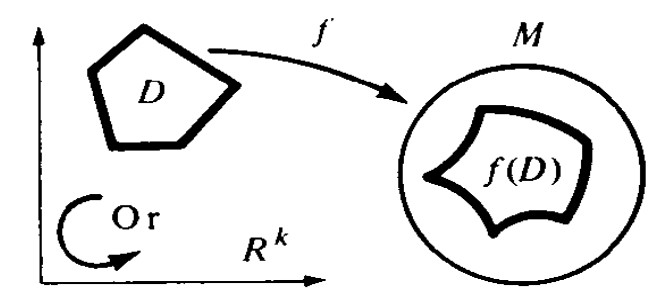
\includegraphics[width=0.35\linewidth]{tcc//img/arnold_celula.jpg}
    \caption{Representação de um poliedro singular $k$-dimensional \citep[Figura 150, pg. 184]{Arnold2013-bs}}
\end{figure}

\begin{definition}
    A integral de uma $k$-forma $\omega \in \Omega^k (M)$ sobre uma célula $\sigma = (D, f, Or)$ é dada por:
    \begin{equation*}
        \int_\sigma \omega := \int_D f^* \omega.
    \end{equation*}
    Ademais, se $c_k = \sum m_i \sigma_i$ é uma $k$-cadeia em $M$, então:
    \begin{equation*}
        \int_{c_k} \omega = \sum m_i \int_{\sigma_i} \omega.
    \end{equation*}
\end{definition}

Com a integração de formas sobre cadeias definida, é possível estender os teoremas integrais do cálculo vetorial para teoremas de integração de formas diferenciais sobre variedades. O mais geral deles é o \textit{Teorema de Stokes Generalizado}.

\begin{theorem}[Teorema de Stokes Generalizado]\citep[192-193]{Arnold2013-bs}
    Sejam $c$ uma $k$-cadeia em $M$ e $\partial c$ o seu bordo. Para $\omega$ uma $(k-1)$-forma em $M$, tem-se:
    \begin{equation*}
        \int_c d \omega = \int_{\partial c} \omega.
    \end{equation*}
\end{theorem}

A intuição por trás do teorema generalizado segue a mesma do teorema tradicional do cálculo vetorial: integrar o diferencial de um operador em um espaço é o mesmo que integrar o operador no bordo desse espaço.

Duas implicações imediatas do Teorema Generalizado vem da integração sobre formas fechadas e sobre formas exatas.

\begin{corollary}\label{corolario:integral_formas_fechadas}
    Se $\omega \in \Omega^k (M)$ é fechada, então $\int_{\partial c} \omega = 0$.
\end{corollary}

\begin{corollary}
    Se $\eta \in \Omega^k (M)$ é exata, então $\int_{\partial c} \eta = 0$.
\end{corollary}

Um último conceito utilizado em mecânica hamiltoniana é o de \textit{invariante integral}.

\begin{definition}
    Uma $k$-forma diferencial $\omega$ é dita um \textbf{invariante integral} de uma aplicação diferenciável $g: M \to M$ se para qualquer $k$-cadeia $c$ tem-se:
    \begin{equation*}
        \int_{gc} \omega = \int_c \omega.
    \end{equation*}
\end{definition}

%%%%%%%%%%%%%%%%%%%%%%%%%%%%%%%%%%%%%%%%%%%%%%%%%%%%%%%%%%%%%%%%%%%%%
% ESPACOS VETORIAIS SIMPLETICOS
%%%%%%%%%%%%%%%%%%%%%%%%%%%%%%%%%%%%%%%%%%%%%%%%%%%%%%%%%%%%%%%%%%%%%
\subsection{Espaços vetoriais simpléticos}
Iniciando o percurso na geometria simplética, trataremos de espaços vetoriais simpléticos, pois a extensão para outros espaços será mais simples. Seja $V$ um espaço vetorial $m$-dimensional sobre $\R$ e $\Omega \in \Lambda^2(V)$ uma 2-forma.

\begin{theorem}\label{teorema:standard_basis_symplectic}\citep{silva_lectures_2001}
    Existem vetores $\vet u_1, ..., \vet u_k$, $\vet e_1, ..., \vet e_n$, $\vet f_1, ..., \vet f_n$ que formam uma base de $V$ tais que
    \begin{align*}
        &\Omega(\vet u_i, \vet v) = 0,  &\forall i, \forall v \in V, \\
        &\Omega(\vet e_i, \vet e_j) = 0 = \Omega(\vet f_i, \vet f_j), &\forall i, j, \\
        &\Omega(\vet e_i, \vet f_j) = \delta_{ij}, &\quad \forall i, j,
    \end{align*}
    onde para $U = \{\vet u \in V | \Omega(\vet u, \vet v) = 0, \forall \vet v \in V\}$ tem-se $k=\dim U$, e $2n + k = \dim V$.
\end{theorem}

\begin{observation}
    Em notação matricial com respeito a essa base, podemos escrever:
    \begin{equation*}
        \Omega(\vet u,\vet v) = \vet u^t \begin{bmatrix}
            \vet 0 & \vet 0 \\ \vet 0 & \bm \Omega
        \end{bmatrix}
        \vet v,
    \end{equation*}
    onde $\bm \Omega = \begin{bmatrix}
        \bm 0 & \bm I \\ - \bm I & \bm 0
    \end{bmatrix}$ é a matriz simplética apresentada anteriormente.
\end{observation}

\begin{definition}
    A aplicação $\tilde \Omega: V \to V^*$ é a 1-forma definida por $\tilde \Omega (\vet v)(\vet u) = \Omega(\vet v,\vet u)$.
\end{definition}

\begin{definition}
    Dizemos que uma 2-forma geral $\Omega$ é \textbf{simplética} (ou \textbf{não degenerada}) se $\tilde \Omega$ é bijetiva, i.e., $\ker \tilde \Omega = \{0\}$. A aplicação $\Omega$ então é denominada como uma \textbf{estrutura simplética linear} sobre $V$, e $(V, \Omega)$ é chamado um \textbf{espaço vetorial simplético}.
\end{definition}

\begin{observation}
    Veja que $\ker \tilde \Omega = U$, então quando $\tilde \Omega$ é bijetiva, $\dim U = k = 0$, logo $\dim V = 2n$, portanto $V$ sempre tem dimensão par. Além disso, pelo teorema \ref{teorema:standard_basis_symplectic}, um espaço vetorial simplético $(V, \Omega)$ tem base $\vet e_1, ..., \vet e_n, \vet f_1, ..., \vet f_n$ satisfazendo
    \begin{equation*}
        \Omega(\vet e_i, \vet f_j) = \delta_{ij}, \quad \Omega(\vet e_i,\vet e_j) = 0 = \Omega(\vet f_i,\vet f_j).
    \end{equation*}
    Por fim, a notação matricial fica reduzida:
    \begin{equation*}
        \Omega(\vet u,\vet v) = \vet u^t \bm \Omega \vet v.
    \end{equation*}
\end{observation}

Diante de uma estrutura sobre um espaço vetorial, cabe perguntar que tipo de funções preservam tal estrutura. Estas funções são chamadas de \textit{simplectomorfismos}.

\begin{definition}
    Um \textbf{simplectomorfismo} $\varphi$ entre dois espaços vetoriais simpléticos $(V, \Omega)$ e $(V', \Omega')$ é um isomorfismo linear $\varphi: V \xrightarrow{\sim} V'$ tal que
    \begin{equation*}
        \varphi^* \Omega' = \Omega, 
    \end{equation*}
    onde $(\varphi^* \Omega')(\vet u,\vet v) = \Omega'(\varphi(\vet u),\varphi(\vet v))$. Se um simplectomorfismo existe, $(V, \Omega)$ e $(V', \Omega')$ são ditos \textbf{simplectomorfos}.
\end{definition}

Ser \textbf{simplectomorfo} é uma relação de equivalência no conjunto de todos os espaços vetoriais de mesma dimensão par. Isso vai além, pois podemos definir um \textbf{protótipo de espaço vetorial simplético} $(\R^{2n}, \Omega_0)$ tal que $\Omega_0$ tem a base
\begin{equation*}
    e_i = (\delta_{i,j})_{j=1,...,2n},
    \quad
    f_i = (\delta_{n+i,j})_{j=1,...,2n},
    \quad
    i = 1, ..., n,
\end{equation*}
e do teorema \ref{teorema:standard_basis_symplectic} decorre que qualquer espaço vetorial simplético $(V, \Omega)$ de dimensão $2n$ é simplectomorfo ao espaço $(\R^{2n}, \Omega_0)$. Então, ter a mesma dimensão par positiva também classifica classes de equivalência para a relação de ser simplectomorfo, de forma que todos os espaços simpléticos de mesma dimensão são simplectomorfos \citep[6]{silva_lectures_2001}.


%%%%%%%%%%%%%%%%%%%%%%%%%%%%%%%%%%%%%%%%%%%%%%%%%%%%%%%%%%%%%%%%%%%%%
% VARIEDADES SIMPLETICAS
%%%%%%%%%%%%%%%%%%%%%%%%%%%%%%%%%%%%%%%%%%%%%%%%%%%%%%%%%%%%%%%%%%%%%
\subsection{Variedades simpléticas}

Tomando uma variedade $M$ e um ponto $\vet p \in M$, o espaço tangente $T_{\vet p} M$ é um espaço vetorial. Uma vez que seja possível construir uma base simplética para uma estrutura $\omega$ em todo o fibrado tangente $TM$, $(T M, \omega)$ é um espaço vetorial simplético, e dizemos que $M$ admite uma \textbf{estrutura quase-simplética}.

É necessária uma restrição a mais para que $\omega$ seja uma estrutura simplética sobre $M$: $\omega$ deve ser fechado. Nesse caso, $\omega$ é dito uma \textbf{forma diferencial simplética} (ou simplesmente \textbf{forma simplética}) e com isso, podemos definir variedades simpléticas.

\begin{definition}
    Uma \textbf{variedade simplética} é um par $(M, \omega)$, onde $M$ é uma variedade e $\omega$ é uma forma simplética.
\end{definition}

Também é possível estender o conceito de \textit{simplectomorfismo} através de \textit{pullbacks}.

\begin{definition}[Simplectomorfismo]\label{def:simplectomorfismo}
    Sejam $(M_1, \omega_1)$ e $(M_2, \omega_2)$ variedades simpléticas e $\varphi: M_1 \to M_2$ um difeomorfismo. Dizemos que $\varphi$ é um \textbf{simplectomorfismo} se $\varphi^* \omega_2 = \omega_1$, onde $\varphi^*$ é o operador de \textbf{pullback}:
    \begin{equation*}
        (\varphi^* \omega_2)_{\vet p}(\vet u,\vet v) = (\omega_2)_{\varphi(\vet p)} (d \varphi_{\vet p}(\vet u), d \varphi_{\vet p}(\vet v)),
    \end{equation*}
    para cada $\vet u, \vet v \in T_{\vet p} M_1$, para cada $\vet p \in M_1$. 
\end{definition}

Uma implicação imediata da definição de simplectomorfismo é a invariância do volume.

\begin{theorem}\label{teorema:simplectomorfismo_invariante_integral}
    Se $g: M \to M$ é uma aplicação diferenciável, então $g$ é um simplectomorfismo se e somente se a forma simplética $\omega$ é um invariante integral de $g$.
\end{theorem}
\begin{Proof}
    Para a ida ($\Rightarrow$), veja que para uma $2$-cadeia $c$ tem-se:
    \begin{equation*}
        \int_{gc} \omega = \int_{c} g^* \omega = \int_{c} \omega.
    \end{equation*}
    Para a volta ($\Leftarrow$), temos que:
    \begin{equation*}
        \int_{gc} \omega = \int_{c} \omega
        \Longrightarrow
        \int_{c} g^* \omega = \int_{c} \omega
        \quad \therefore \quad
        g^* \omega = \omega.
    \end{equation*}
\end{Proof}

Uma vez que $\omega$ é uma 2-forma simplética, $\omega$ é o diferencial de uma 1-forma, e assim é definida pelo produto exterior de 1-formas. Isso significa que $\omega$ corresponde a um volume em seu domínio, então um simplectomorfismo é um difeomorfismo que conserva um volume em sua trajetória.

O conceito de espaços \textbf{simplectomorfos} é idêntico ao caso linear. Ainda, se tomamos $\R^{2n}$ com coordenadas $x_1, ..., x_n, y_1, ..., y_n$, a forma
\begin{equation*}
    \omega_0 = \sum_{i=1}^{n} dx_i \wedge dy_i
\end{equation*}
é simplética e logo $(\R^{2n}, \omega_0)$ é um espaço simplético, e da mesma forma que toda variedade de dimensão $n$ é localmente ``parecida'' com $\R^n$, toda $2n$-variedade simplética é localmente ``parecida'' com $(\R^{2n}, \omega_0)$, no sentido de que toda variedade $(M^{2n}, \omega)$ é localmente simplectomorfa a $(\R^{2n}, \omega_0)$. Isso decorre do \textbf{teorema de Darboux} e foge do escopo deste trabalho, mas os detalhes podem ser encontrados em \cite[7]{silva_lectures_2001}.

Uma forma prática de caracterizar simplectomorfismos dentro de um mesmo espaço é através da fórmula mágica de Cartan, o teorema \ref{teorema:formula_magica_cartan}.

\begin{theorem}\label{teorema:simplectomorfismo_e_lie}
    Sejam $X$ um campo vetorial suave em uma variedade simplética $(M, \omega)$, com fluxo associado $\varphi_t$ para algum ponto $\vet p \in M$. O fluxo $\varphi_t$ é um simplectomorfismo se, e só se, $\mathcal L_X \omega = 0$.
\end{theorem}
\begin{Proof}
    Pela definição \ref{def:simplectomorfismo}, queremos provar que $\varphi_t^* \omega = \omega \Leftrightarrow \mathcal L_X \omega = 0$.
    
    Para o lado ($\Rightarrow$), se $\varphi_t$ é um simplectomorfismo, tem-se por definição:
    \begin{equation*}
        \mathcal L_X \omega = \der{}{t}\bigg\rvert_{t=0} \varphi_t^* \omega
        = \der{}{t}\bigg\rvert_{t=0} \omega = 0.
    \end{equation*}
    Já para ($\Leftarrow$) Uma vez que $\varphi_{s_1} \circ \varphi_{s_2} = \varphi_{s_1 + s_2}$ (pela definição de fluxo), segue que
    \begin{equation*}
        \varphi_\lambda^* (\mathcal L_X \omega)
        = \varphi_\lambda^* \left(\der{}{t}\bigg\rvert_{t=0} \varphi_t^* \omega\right) 
        = \der{}{t}\bigg\rvert_{t=0} \varphi_{t+h}^* \omega
        = \der{}{t}\bigg\rvert_{t=\lambda}\varphi_t \omega.
    \end{equation*}
    Por hipótese, temos que $\mathcal L_X \omega = 0$, então
    \begin{equation*}
        \der{}{t}\bigg\rvert_{t=\lambda} \varphi_t^* \omega = 0, \quad \forall \lambda \in \R,
    \end{equation*}
    o que significa que a aplicação $\mu(\lambda) = \varphi_\lambda^* \omega$ é constante. Veja que
    \begin{equation*}
        \mu(0) = \varphi_0^* \omega = \omega \circ \varphi_0 = \omega 
        \Rightarrow
        \varphi_t^* \omega = \omega.
    \end{equation*}
\end{Proof}

Uma variedade simplética já conhecida neste momento é o \textit{fibrado cotangente} $T^* M$. Para coordenadas locais $(\vet q, \vet p)$, tomamos uma 1-forma $\omega^1 = \vet p d \vet q$. A partir disso, uma 2-forma exata natural é $\omega^2 = d \omega^1$, e que por ser exata é fechada, e portanto simplética. A 2-forma $\omega^2$ é dada por
\begin{equation*}
    \omega(f,g) = (d \vet q \wedge d \vet p)(f,g) = \derpar{f}{\vet q} \derpar{g}{\vet p} - \derpar{f}{\vet p} \derpar{g}{\vet q} = \nabla^t f \bm \Omega \nabla g,
\end{equation*}
onde $\bm \Omega$ é a matriz simplética. Com isso, agora é possível estudar os campos hamiltonianos e sua relação com a geometria simplética.

\subsection{Campos hamiltonianos}

Os campos hamiltonianos são um tipo de campo simplético com uma propriedade a mais: a 2-forma é exata.

\begin{definition}[Campo hamiltoniano]
    Sejam $X$ um espaço vetorial em uma variedade simplética $(M, \omega)$ e $H: M \to \R$ uma função suave. Dizemos que $X$ é um \textbf{campo hamiltoniano} se $\iota_X \omega = dH$ é exato. O campo $X$ é denotado por $X_H$ devido a sua relação com $H$ e dizemos que $(M, \omega, H)$ é um \textbf{sistema hamiltoniano}.
\end{definition}

Conforme o teorema \ref{teorema:simplectomorfismo_e_lie}, é fácil ver que todo campo hamiltoniano é necessariamente simplético, ou seja, o fluxo associado é um simplectomorfismo.

\begin{corollary}
    Todo campo hamiltoniano $X_H$ é simplético.
\end{corollary}
\begin{Proof}
    Pela fórmula de Cartan, temos que
    \begin{equation*}
        \mathcal L_{X_H} \omega = \iota_{X_H} (d \omega) + d (\iota_{X_H} \omega) = 0 + d(dH) = 0, 
    \end{equation*}
    pois $d \omega = 0$ ($\omega$ é simplético) e $\iota_{X_H} \omega = dH$. Pelo teorema \ref{teorema:simplectomorfismo_e_lie}, o fluxo $\varphi_t$ associado ao campo hamiltoniano $X_H$ é um simplectomorfismo.
\end{Proof}

Uma vez que o fluxo hamiltoniano é simplético, vale o teorema \ref{teorema:simplectomorfismo_invariante_integral}, então há também a conservação do volume. Isso é uma forma simplética de expressar o que já havia sido visto pelo teorema \ref{teorema:hamiltoniano_volume}, também chamado de \textbf{teorema de Liouville}. Essa conservação está ligada diretamente com a existência de integrais primeiras, e em particular $H$  é uma integral primeira para o fluxo $\varphi_t$.

\begin{proposition}
    A função $H$ é uma integral primeira do fluxo hamiltoniano $\varphi_t$.
\end{proposition}
\begin{Proof}
    Pela definição de $dH$, temos que:
    \begin{equation*}
        dH(X_H) = \iota_{X_H} \omega (X_H) = \omega(X_H, X_H) = 0.
    \end{equation*}
\end{Proof}

De fato, toda integral primeira do fluxo hamiltoniano terá campo tangente anulado por $dH$.

\begin{proposition}
    Seja $f$ uma função em $M$. $f$ é uma integral primeira para o fluxo hamiltoniano $\varphi_t$ se, e somente se, $dH(X_f) = 0$, onde $X_f = df$.
\end{proposition}
\begin{Proof}
    Se $f$ é uma integral primeira para $\varphi_t$, então
    \begin{equation*}
        \der{}{t} f(\varphi_t) = X_f \der{}{t} \varphi_t = dH (X_f) = 0.
    \end{equation*}
    A volta é análoga.
\end{Proof}

Ademais, um operador bastante presente na mecânica hamiltoniana é o \textit{colchete de Poisson}.

\begin{definition}
    Seja $(M, \omega)$ uma variedade simplética. O colchete de Poisson $\{\cdot,\cdot\}$ é um operador bilinear definido por
    \begin{equation*}
        \{f, g\}
        = - \iota_{X_f} \iota_{X_g} \omega 
        = \omega(X_f, X_g)
        = (\nabla f)^t \bm \Omega (\nabla g).
    \end{equation*}
\end{definition}

Com essa notação, é possível reescrever o resultado anterior sobre integrais primeiras: uma função $f$ é uma integral primeira para o fluxo hamiltoniano com função hamiltoniana $H$ se, e só se, $\{H, f\} = 0$. Além disso, se $f$ é uma função no espaço de fases, então
\begin{equation*}
    \der{}{t} f = \derpar{f}{t} + \{f, H\}.
\end{equation*}

Por fim, por maior que seja a diversidade de funções hamiltonianas, as que interessam neste trabalho são as cujo campo $X_H$ é dado por
\begin{equation*}
    X_H = \bm \Omega dH,
\end{equation*}
onde $\bm \Omega$ é a matriz simplética, e o espaço em questão é $(T^*M, \omega^2)$, com coordenadas $(\vet q, \vet p)$ e 2-forma associada. Isso significa, em particular, que
\begin{equation*}
    \{f, g\} = Df^t \bm \Omega Dg = \sum_i \derpar{f}{q_i}\derpar{g}{p_i} - \derpar{f}{p_i}\derpar{g}{q_i}.
\end{equation*}

Com essa notação, também é possível reescrever as equações de Hamilton (conforme teorema \ref{teorema:equacoes_hamilton}):
\begin{equation}\label{eq:poisson_hamilton_equacoes}
    \begin{cases}
        \dvet q(t) = \{\vet q, H\}, \\
        \dvet p(t) = \{\vet p, H\},
    \end{cases}
    \quad \text{ ou } \quad
    \dot \varphi(t) = \{\varphi, H\},
\end{equation}
onde $\varphi(t) = (\vet q(t), \vet p(t))$ é o fluxo hamiltoniano. Além disso, qualquer sistema de \textit{coordenadas canônicas} pode ser identificado através do colchete de Poisson: se $(\vet u, \vet v)$ é um par de coordenadas canônicas então
\begin{equation}\label{eq:poisson_coordenadas_canonicas}
    \{\vet u_a, \vet u_b \} = 0,
    \quad
    \{\vet v_a, \vet v_b \} = 0,
    \quad
    \{\vet u_a, \vet v_b \} = \delta_a^b.
\end{equation}
Observe que estas são as mesmas propriedades esperadas para uma \textit{base} de um espaço vetorial simplético, como no teorema \ref{teorema:standard_basis_symplectic}.

%%%%%%%%%%%%%%%%%%%%%%%%%%%%%%%%%%%%%%%%%%%%%%%%%%%%%%%%%%%%%%%%%%%%%
% TRANSFORMACOES CANONICAS
%%%%%%%%%%%%%%%%%%%%%%%%%%%%%%%%%%%%%%%%%%%%%%%%%%%%%%%%%%%%%%%%%%%%%
\subsection{Transformações canônicas}
Nesta última seção, é melhor explorado o significado do teorema \ref{teorema:simplectomorfismo_invariante_integral}. Os simplectomorfismos, caracterizados por terem a forma simplética como invariante integral, são também chamados de \textit{transformações canônicas}. A preservação das equações de Hamilton é uma consequência sob a aplicação de transformações canônicas, o que às vezes é mais prático de se testar do que a teoria simplética vista. Nesta seção, considere uma aplicação $\vet z \mapsto \vet w$, onde $\vet z = (\vet q, \vet p)$ e $\vet w = (\vet Q, \vet P)$, e dois campos hamiltonianos $V_H$ e $V_K$ associados de maneira respectiva.

\begin{definition}[Transformação canônica]
    Dizemos que a transformação $\vet z \mapsto \vet w$ é \textbf{canônica} se $H(\vet z) = K(\vet z'(\vet z))$ e se preserva as equações de Hamilton, isto é:
    \begin{equation*}
        \dvet z = \bm \Omega \nabla_{\vet z} H
        \longrightarrow
        \dvet z' = \bm \Omega \nabla_{\vet z'} K.
    \end{equation*}
\end{definition}

A partir da definição de transformação canônica, é possível deduzir uma forma prática de validar a simpleticidade de aplicações.

\begin{theorem}\label{teorema:simpleticidade_matricial}
    Uma aplicação $\vet z \mapsto \vet w$ é canônica se, e só se, sua matriz jacobiana
    \begin{equation*}
        \bm J = \derpar{(\vet Q, \vet P)}{(\vet q, \vet p)}
    \end{equation*}
    atende a seguinte condição:
    \begin{equation}\label{eq:simpleticidade_matricial_1}
        \bm J \bm \Omega \bm J^t = \bm \Omega.
    \end{equation}
\end{theorem}
\begin{Proof}
    Uma vez que $H(\vet z) = K(\vet w(\vet z))$, então $\nabla_{\vet z} H = \bm J^t \nabla_{\vet w} K$. Dessa forma,
    \begin{equation*}
        \dvet w 
        = \bm J \dvet z 
        = \bm J (\bm \Omega \nabla_{\vet z} H)
        = \bm J \bm \Omega \bm J^t \nabla_{\vet w} K
        = \bm \Omega \nabla_{\vet w} K,
    \end{equation*}
    sendo a última passagem por definição. Assim, a equação \ref{eq:simpleticidade_matricial_1} é necessária para que a aplicação seja canônica e vice-versa. É fácil ver que uma vez que esteja atendida, também é suficiente para garantir que $\vet z \mapsto \vet w$ se encaixa na definição de aplicação canônica.
\end{Proof}

\begin{corollary}
    Uma formulação equivalente a (\ref{eq:simpleticidade_matricial_1}) é:
    \begin{equation}\label{eq:simpleticidade_matricial_2}
        \bm J \bm \Omega \bm J^t \bm \Omega^t = \bm I.
    \end{equation}
\end{corollary}
\begin{Proof}
    A matriz $\bm \Omega$ é ortonormal, então $\bm \Omega^{-1} = \bm \Omega^t$.
\end{Proof}

Pelo teorema \ref{teorema:simpleticidade_matricial}, a aplicação ser canônica equivale a preservar o colchete de Poisson: para qualquer $u, v$, temos
\begin{equation*}
    \{ u, v \}_{\vet z}
    = (\nabla_{\vet z} u)^t \bm \Omega (\nabla_{\vet z} v)
    = (\nabla_{\vet w} u)^t \bm J \bm \Omega \bm J^t (\nabla_{\vet w} v)
    = (\nabla_{\vet w} u)^t \Omega (\nabla_{\vet w} v)
    = \{u, v \}_{\vet w}.
\end{equation*}

Mais ainda. A conservação do Parêntese de Poisson significa que a própria forma $\omega$ do sistema hamiltoniano está sendo conservada. Pela definição (\ref{def:simplectomorfismo}), as transformações canônicas são simplectomorfismos.

Com essa nova notação e novos conceitos, as equações de Hamilton no teorema \ref{teorema:equacoes_hamilton} ganham uma base teórica mais sólida, se definindo sobre espaços com estruturas bem definidas e específicas o suficiente para fornecer resultados numéricos; observar a variação numérica de um valor que deveria ser conservado teoricamente durante uma trajetória fornece informações sobre a razoabilidade de uma simulação, por exemplo. Isso será visto com mais detalhes no capítulo \ref{capitulo:metodos_numericos}.